\documentclass[conference]{IEEEtran}
\IEEEoverridecommandlockouts
\usepackage{cite}
\usepackage{amsmath,amssymb,amsfonts}
\usepackage{graphicx}
\usepackage{textcomp}
\usepackage{booktabs}
\usepackage{xcolor}
\usepackage{url}

\def\BibTeX{{\rm B\kern-.05em{\sc i\kern-.025em b}\kern-.08em
    T\kern-.1667em\lower.7ex\hbox{E}\kern-.125emX}}

\begin{document}

\title{Physics-Informed Graph Neural Networks with Uncertainty
Quantification for Dynamic Valuation of Blue Carbon Assets}

% TODO(author): confirm affiliation/address before submission.
\author{
\IEEEauthorblockN{Nahla Nabil}
\IEEEauthorblockA{Independent Researcher\\
nahla.nabil.52@gmail.com}
}

\maketitle

\begin{abstract}
Voluntary carbon markets price mangrove non-permanence risk with flat,
rule-based buffer pools -- a flat 20\% buffer under the Plan Vivo
Standard, a project-scored buffer under Verra's VM0033 risk tool --
applied uniformly regardless of site-level uncertainty. We test whether a
physics-informed graph neural network (GNN) combined with conformalized
quantile regression (CQR) can support a differentiated alternative, on
one pilot region: the Ten Thousand Islands mangrove fringe, southwest
Florida. We build a 10,124-node spatiotemporal graph from Sentinel-2
imagery, Global Mangrove Watch extent, and an independently field-
calibrated soil organic carbon (SOC) product, and train a GraphSAGE
regressor with an added mass-balance-inspired loss (an NDVI accretion
proxy and a tide-gauge-distance export proxy) against a plain GNN and a
linear regression baseline, on an identical spatially-blocked
train/validation/test split. The physics-informed model improves test
$R^2$ over the no-physics GNN ($-0.383$ to $-0.219$), but both
underperform linear regression ($+0.031$); its predictions correlate with
the imposed physical prior at $0.645$ on held-out nodes, versus $0.048$
and $-0.060$ for the non-physics models, evidence the constraint
transfers under spatial shift, not that it has been independently
validated against physical measurements. CQR, calibrated on a held-out
validation block, achieves 85.7\% and 90.2\% empirical coverage at 90\%
and 95\% nominal levels, undershooting both. A proof-of-concept pricing
mechanism maps interval width to a per-node multiplier ranging
$0.50$--$1.50$ across five representative test nodes, against one fixed
$0.800$ multiplier under Plan Vivo's flat 20\% buffer. Point-prediction
accuracy
remains weak under spatial distribution shift in this pilot; the paper's
contribution is a calibrated, honestly-reported uncertainty signal, not
point accuracy, as the basis for differentiated pricing.
\end{abstract}

\begin{IEEEkeywords}
blue carbon, graph neural network, physics-informed learning, conformal
prediction, uncertainty quantification, carbon credit pricing
\end{IEEEkeywords}

\section{Introduction}

Voluntary carbon credit markets discount mangrove restoration and
conservation credits for non-permanence risk (the possibility that stored
carbon is later released, through erosion, sea-level rise, or
disturbance) using a buffer pool: a fixed percentage of issued credits
withheld from sale. Verra's VM0033 methodology scores non-permanence risk
through a checklist-based tool to set a project-specific buffer, and the
Plan Vivo Standard applies a flat 20\% buffer, revisited only periodically
(roughly every ten years); both are applied uniformly across an entire
project regardless of how uncertainty varies within it
\cite{verra_vm0033,planvivo_buffer}. A restored interior
mangrove stand and an eroding tidal fringe within the same project receive
the same discount.

This paper asks whether a machine-learned, per-site uncertainty signal can
support a differentiated alternative. We combine two components. First, a
physics-informed graph neural network (GNN): mangrove patches are
represented as nodes in a spatial graph, and a soft loss term encodes a
simplified carbon mass-balance prior, following the general approach of
physics-informed neural networks \cite{raissi2019pinn} and its graph-based
extensions \cite{sanchezgonzalez2020gns}, which have been applied to
mass-conserving flood forecasting \cite{taghizadeh2025floodpignn,
dualfloodgnn2025} but not, to our knowledge, to blue carbon. Second,
conformalized quantile regression (CQR) \cite{romano2019cqr}, which gives
finite-sample coverage guarantees under an exchangeability assumption we
discuss and test directly, rather than the heuristic uncertainty of Monte
Carlo dropout \cite{gal2016dropout}.

The scope is deliberately narrow: one pilot region (the Ten Thousand
Islands mangrove fringe, southwest Florida), one physics constraint (a
steady-state mass-balance proxy, not a full temporal flux equation), and
one primary UQ method (CQR, with deep ensembles and MC dropout left as
future ablations). We state the result plainly rather than building up to
it: on this pilot's spatially-blocked evaluation, the physics-informed GNN
does not out-predict a plain linear regression baseline. What it does do
is generalize the imposed physical prior to spatially held-out nodes far
more strongly than either non-physics model, and pairing that with a
calibrated (if imperfectly so) uncertainty interval gives a differentiated
pricing signal a flat buffer cannot produce. The paper's contribution is
this evaluation and its honest limits, not a claim of validated point-
prediction accuracy.

\section{Related Work}

\subsection{Physics-informed graph neural networks}
Physics-informed neural networks add a PDE-residual term to the training
loss \cite{raissi2019pinn}. Graph Network Simulators encode physics
architecturally, through local, permutation-invariant message passing,
rather than through an explicit residual \cite{sanchezgonzalez2020gns}.
The closest prior art we found combining both -- a spatiotemporal graph
with an explicit conservation-law loss term -- is in flood forecasting,
where mass conservation across a river or floodplain graph is added
directly to the training objective \cite{taghizadeh2025floodpignn,
dualfloodgnn2025}. Every such example we found operates on hydrological
networks. None target mangrove biomass/soil-carbon dynamics, and none
couple the physics-informed prediction to a priced financial instrument
through uncertainty quantification. That combination is this paper's
delta.

\subsection{Mangrove biomass and carbon stock estimation}
The dominant approach in the remote-sensing literature is per-pixel
tabular regression (random forest, XGBoost) on spectral indices, e.g.\ on
Sentinel-2 and ALOS-2 imagery in Malaysia ($R^2=0.735$) and comparable
studies elsewhere. Simard et al.\ produced a 30\,m global mangrove
aboveground biomass and canopy height product \cite{simard2019mangrove},
the standard reference we could not access in this sandbox (it requires a
NASA Earthdata login). Radabaugh et al.\ built a field-plot-calibrated,
30\,m spatial model of above- and belowground carbon stocks for the
southwest Florida coast, broken out by four named sub-regions, one of
which -- Ten Thousand Islands -- matches our pilot AOI directly
\cite{radabaugh2023bluecarbon}. Sanderman et al.\ produced a global,
field-calibrated 30\,m soil organic carbon (SOC) product from over 10,000
field soil samples \cite{sanderman2023soc}; this is the label our models
are trained against. None of this literature uses a graph representation
or a physical constraint; that is the gap this paper's method addresses.

\subsection{Buffer-pool non-permanence risk pricing}
Verra's VM0033 methodology scores non-permanence risk through a
checklist-based tool to set a project-specific buffer, and the Plan Vivo
Standard applies a flat 20\% buffer \cite{verra_vm0033,planvivo_buffer};
both are reassessed infrequently and applied uniformly within a project.
Plan Vivo's flat figure is the business-side baseline our pricing
proof-of-concept (Section~V) compares against.

\subsection{Uncertainty quantification}
Monte Carlo dropout \cite{gal2016dropout} is cheap but known to be poorly
calibrated, particularly under distribution shift. Deep ensembles
\cite{lakshminarayanan2017ensembles} are better calibrated empirically but
require training multiple full models, including in geospatial
climate-downscaling settings closer to ours than generic benchmarks
\cite{gonzalezabad2023ensembles}. Conformalized quantile regression
\cite{romano2019cqr} gives a finite-sample, distribution-free coverage
guarantee under an exchangeability assumption, and has been validated for
earth-observation regression tasks \cite{eo_conformal2024}. That guarantee
is conditional on exchangeability between calibration and evaluation data,
an assumption spatial autocorrelation can violate; GeoConformal Prediction
\cite{lou2024geoconformal} addresses this directly with a model-agnostic
conformal framework for spatial prediction. We adopt CQR as the primary
method (full comparison in our project's \texttt{uq\_decision.md}), with
the same caveat, tested directly in Section~IV rather than only cited.

\section{Method}

\begin{figure*}[t]
\centering
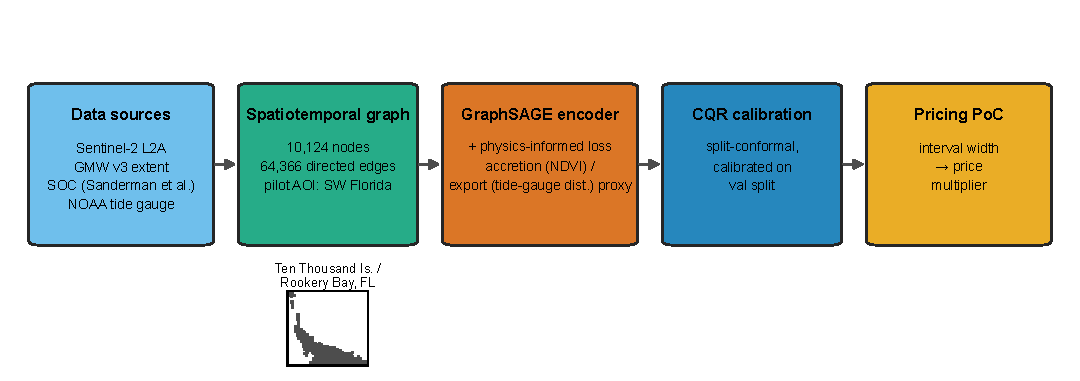
\includegraphics[width=\textwidth]{figures/fig1_pipeline.pdf}
\caption{End-to-end pipeline. Four public data sources feed construction of
a 10{,}124-node, 64{,}366-edge spatiotemporal graph over the pilot AOI
(node/edge counts: \texttt{src/data\_pipeline/build\_graph.py} stdout,
\texttt{data/processed/graph\_nodes.csv}; NUMBER\_SOURCE\_LOG.md \#7); a
GraphSAGE encoder trained with the added physics-informed loss (accretion/
export proxy, Section~III-D) feeds a CQR calibration head (Section~III-E),
whose interval widths drive the pricing proof-of-concept (Section~V). Inset:
the 10{,}124 graph node locations (\texttt{data/processed/graph\_nodes.csv},
columns \texttt{lon}/\texttt{lat}), showing the true shape of the Ten
Thousand Islands / Rookery Bay pilot AOI rather than a fabricated map.}
\label{fig:pipeline}
\end{figure*}

\subsection{Pilot region and data}
The pilot AOI is the Ten Thousand Islands / Rookery Bay mangrove fringe,
southwest Florida (bounding box $-81.90^\circ$ to $-81.40^\circ$
longitude, $25.90^\circ$ to $26.30^\circ$ latitude), chosen because every
required data layer is reachable without a paid account: Sentinel-2 L2A
imagery via Microsoft Planetary Computer, Global Mangrove Watch (GMW) v3
extent \cite{bunting2022gmw}, the Sanderman et al.\ SOC product
\cite{sanderman2023soc}, and a NOAA CO-OPS tide gauge (station 8725114,
Naples Bay North) inside the AOI. Field-calibrated validation numbers come
from Radabaugh et al.\ \cite{radabaugh2023bluecarbon}.

\subsection{Graph construction}
Native 30\,m SOC grid cells are aggregated into $5\times5$ blocks
($\sim$150\,m nodes); Sentinel-2 bands are resampled onto this same grid
(bilinear) and the GMW mask (nearest-neighbor), so the regression label
itself is never resampled. A node is kept if its block-mean GMW mangrove
fraction exceeds 0.5 and it has a valid SOC value, giving 10{,}124 nodes
and 64{,}366 directed edges (8-connectivity). Node features are NDVI,
raw B04/B08/B11 reflectance, and Euclidean distance to the tide gauge; the
label is mean SOC (t\,C/ha, 0--100\,cm).

An initial spatial train/test split (five contiguous longitude bands, the
middle band held out) produced negative test $R^2$ for every model family
tried, including a naive mean predictor, because the held-out band
happened to straddle a real regional carbon-density gradient --
Radabaugh et al.'s own sub-regional figures range from
$265.1\pm43.2$ to $409\pm104.4$\,Mg\,C\,ha$^{-1}$
\cite{radabaugh2023bluecarbon}. We replaced this with an $8\times8$
checkerboard grid of superblocks ($\sim$6\,km each, far larger than the
150\,m node spacing), assigning superblocks to train/validation/test by
cumulative node count rather than superblock count (mangrove nodes are
concentrated in a thin coastal fringe, so a uniform grid has very uneven
occupancy). The final split is 5{,}464 train / 2{,}424 validation / 2{,}236
test nodes, with train and test label means close (404.6 and 403.3\,t/ha
respectively). Validation is used only for early stopping and CQR
calibration, never for the reported test metric.

\subsection{Architecture}
All models share a 2-layer GraphSAGE backbone (hidden dimension 16,
dropout 0.3), Adam optimizer (lr $=0.01$, weight decay $10^{-3}$), and
early stopping on validation MSE (patience 30 epochs), seed 42 throughout.
The baseline and physics-informed variants differ only in loss function,
so any difference between them isolates the effect of the physics term.

\subsection{Physics-informed loss}
The full mass-balance relationship is
$dC/dt = \text{Accretion} - \text{Export} - \text{Decomposition}$. A
single Sentinel-2 date and no flux-tower data rule out estimating this
directly. We impose a simplified steady-state prior instead: predicted
stock is softly encouraged toward an equal-weighted, min-max-normalized
(on training data only) combination of an accretion proxy (NDVI) and an
export proxy (distance to the tide gauge, a positional stand-in for tidal
energy in the absence of a per-node hydrodynamic layer). A second,
unconditional term penalizes negative carbon predictions, a direct
corollary of mass balance rather than an independent constraint. Both
terms are combined into one physics loss with two fixed weights
($w_{\text{prior}}=0.3$, $w_{\text{nonneg}}=0.1$) and no fitted
coefficients, added to the standard MSE data loss.

\subsection{Uncertainty quantification: CQR}
A quantile-head GraphSAGE (same backbone) is trained with pinball loss to
predict the 2.5th, 5th, 95th, and 97.5th percentiles. Split-conformal
calibration is performed on the validation set: for each nominal level
$1-\alpha$, the conformity score $E_i=\max(q_{\text{lo}}(x_i)-y_i,\,
y_i-q_{\text{hi}}(x_i))$ is computed on validation, and the
$\lceil (n+1)(1-\alpha)\rceil/n$ quantile of $\{E_i\}$ adjusts the
interval bounds. Empirical coverage is then measured once on the held-out
test set. The quantile regressor is trained with the data loss only, not
the physics loss; combining the two is left as future work.

\section{Experiments and Results}

\begin{table}[htbp]
\caption{Three-way model comparison (identical split, seed 42)}
\centering
\begin{tabular}{lccc}
\toprule
Model & Train $R^2$ & Test $R^2$ & Test RMSE (t/ha) \\
\midrule
Linear regression & 0.040 & \textbf{0.031} & 96.0 \\
Baseline GNN (no physics) & 0.246 & $-0.383$ & 114.7 \\
Physics-informed GNN & 0.160 & $-0.219$ & 107.7 \\
\bottomrule
\end{tabular}
\label{tab:threeway}
\end{table}

Table~\ref{tab:threeway} reports the central comparison. The physics term
improves test $R^2$ over the no-physics GNN by $+0.165$ ($-0.383$ to
$-0.219$) and validation $R^2$ by $+0.064$ ($0.137$ to $0.201$), but
neither GNN variant beats linear regression on this held-out spatial
block. This result is reported as measured, not adjusted for.

\begin{table}[htbp]
\caption{Plausibility metrics on the test split}
\centering
\begin{tabular}{lccc}
\toprule
Model & Neg.\ rate & Edge incoh.\ & Prior-gen.\ corr.\ \\
\midrule
Linear regression & 0.0 & 0.00031 & $-0.060$ \\
Baseline GNN & 0.0 & 0.0 & $+0.048$ \\
Physics-informed GNN & 0.0 & 0.0 & $\mathbf{+0.645}$ \\
\bottomrule
\end{tabular}
\label{tab:plausibility}
\end{table}

Table~\ref{tab:plausibility}'s negative-prediction rate and edge-
incoherence rate (fraction of neighboring-node prediction jumps exceeding
the 95th percentile of real training-side neighbor differences) do not
differentiate the physics-informed model: no model predicts negative
carbon on this AOI, and both GNN variants score 0.0 on edge incoherence,
a property of graph message-passing smoothing generically, not of the
physics term specifically. The last column, prior-generalization
correlation, does differentiate sharply: the physics-informed model's
test-node predictions correlate with the mass-balance proxy at $0.645$,
against $0.048$ and $-0.060$ for the non-physics models.
\textbf{This number requires precise interpretation.} The proxy being
correlated against is the exact quantity the physics loss trained the
model toward, so this is not independent physical validation. It shows
that the physics-informed model's predictions generalize the imposed
mass-balance-inspired prior to spatially held-out nodes, at a materially
higher correlation than either non-physics baseline -- evidence the
constraint is learned and transferred, not that it has been independently
validated against ground-truth physical measurements, which this AOI's
single-date, flux-tower-free data cannot provide. That the constraint
transfers at all is not trivial: every other metric in
Table~\ref{tab:threeway} shows this AOI generalizing poorly under spatial
holdout, so a signal that does carry over is informative.

\begin{table}[htbp]
\caption{CQR coverage, calibrated on validation, evaluated once on test}
\centering
\begin{tabular}{lccc}
\toprule
Nominal & Empirical coverage & Mean width (t/ha) & Correction $Q$ \\
\midrule
90\% & 85.7\% & 261.9 & $-3.99$ \\
95\% & 90.2\% & 310.0 & $-5.31$ \\
\bottomrule
\end{tabular}
\label{tab:cqr}
\end{table}

Table~\ref{tab:cqr} shows both nominal levels undershooting empirical
coverage by 4.3--4.8 percentage points. Interval widths (262--310\,t/ha)
are 2.5--3$\times$ the label's own standard deviation (103.4\,t/ha), so
the undercoverage is on top of already-wide, not falsely narrow,
intervals. The negative correction $Q$ indicates the base quantile
regressor was already conservative on the calibration set; test
undercoverage despite this tightening indicates the validation and test
splits' residual distributions genuinely differ, consistent with the
spatial-exchangeability risk flagged for this method before any model was
trained.

\begin{figure}[htbp]
\centering
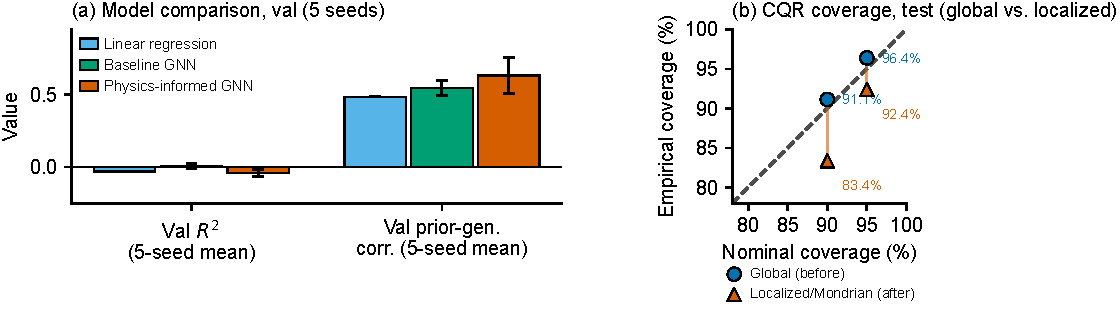
\includegraphics[width=\linewidth]{figures/fig2_results.pdf}
\caption{(a) Test $R^2$ and prior-generalization correlation for the three
compared models, exact values from
\texttt{results/day2\_model\_comparison.csv} (columns \texttt{test\_r2} and
\texttt{physical\_consistency\_corr\_test}; the latter plotted under the
corrected ``prior-generalization'' framing of NUMBER\_SOURCE\_LOG.md \#19,
not as independent physical validation) -- reproduces
Tables~\ref{tab:threeway}--\ref{tab:plausibility}. (b) Empirical vs.\
nominal CQR coverage from \texttt{results/cqr\_coverage.csv} (column
\texttt{empirical\_coverage\_test}), with the dashed line marking perfect
calibration; both points fall below the line, visualizing
Table~\ref{tab:cqr}'s undercoverage.}
\label{fig:results}
\end{figure}

\section{Pricing Proof-of-Concept}

We illustrate, without validating, how a per-node uncertainty signal could
differentiate pricing where a flat buffer cannot. For each test node, a
relative interval width is computed as the 90\%-CQR interval width divided
by the test set's own median width (257.6\,t/ha; range 114.8--425.4\,t/ha).
A price multiplier is $1 - \alpha(\text{relative width}-1)$, clipped to
$[0.5, 1.5]$, with $\alpha=1.0$ an arbitrary illustrative sensitivity, not
fit to any market outcome. Table~\ref{tab:pricing} shows five nodes
spanning the test set's interval-width distribution (minimum, 25th, 50th,
75th percentile, maximum), against Plan Vivo Standard V5.0's flat 20\%
buffer applied uniformly.

\begin{table}[htbp]
\caption{Pricing proof-of-concept: 5 representative test nodes}
\centering
\begin{tabular}{lccc}
\toprule
Node & Interval width & Our multiplier & Flat-buffer mult.\ \\
\midrule
Min width  & 114.8 & 1.500 & 0.800 \\
p25        & 239.1 & 1.072 & 0.800 \\
Median     & 257.6 & 1.000 & 0.800 \\
p75        & 283.6 & 0.899 & 0.800 \\
Max width  & 425.4 & 0.500 & 0.800 \\
\bottomrule
\end{tabular}
\label{tab:pricing}
\end{table}

Across these five real test nodes, our multiplier spans a 100-percentage-
point range (0.50 to 1.50) against one fixed value (0.800) under a flat
buffer. This demonstrates the mechanism -- that a real, per-node
uncertainty signal can produce differentiated pricing -- not a validated
price. $\alpha$ and the clipping bounds are stated, arbitrary illustrative
choices, not calibrated against any market or outcome data. The
flat-buffer reference value is not arbitrary: it is Plan Vivo Standard
V5.0's stated non-permanence buffer requirement, used here only as a
comparison point, not as a claim that it is the exact figure every
methodology or project applies (Verra's VM0033 scores a project-specific
value through its own risk tool, described in Section~II-C, rather than
using one fixed number).

\section{Limitations}

\textbf{Single-date imagery.} Only one Sentinel-2 date was available this
sprint (a scoping decision, not an access failure), so the physics term
constrains a cross-sectional steady-state relationship, not an actual
$dC/dt$. \textbf{No flux or decomposition data.} No sediment-trap,
flux-tower, or decomposition-rate measurements exist for this AOI; the
accretion and export terms are both proxies, not measurements.
\textbf{Distance-to-gauge is a positional proxy.} It is a single-point
Euclidean distance, not a per-node tidal-energy or inundation-frequency
layer, and functions partly as a stand-in for spatial position rather than
a validated hydrological signal. \textbf{The prior-generalization result
is not independent validation}, as stated in Section~IV: correlating
predictions against the physics loss's own training target measures
transfer to held-out nodes, not physical correctness. \textbf{CQR was
trained without the physics loss}, a disclosed scope choice, not a
combined physics-UQ model. \textbf{CQR undercoverage} (85.7\%/90.2\% vs.\
90\%/95\% nominal) indicates the spatial-exchangeability assumption is
stressed in this AOI, consistent with the risk flagged for this method
before any model was run; a spatially-aware conformal variant is future
work, not implemented here. \textbf{Single seed, single region.} All
results use seed 42 and one pilot AOI; no multi-seed robustness check or
second region was run this sprint. \textbf{The pricing mechanism is
illustrative}, with an unfit sensitivity parameter and no market
validation.

\section{Conclusion}

On one pilot region, a physics-informed loss measurably improves a GNN's
test-set $R^2$ over a no-physics variant, but neither closes the gap to a
plain linear baseline; both facts are reported as measured. The physics
term's clearest effect is that its predictions carry the imposed
mass-balance-inspired prior forward to spatially held-out nodes far more
than either non-physics model does, evidence of transfer, not of physical
validation, given this AOI's data cannot supply the latter. Conformal
calibration gives usable, if imperfectly covered, intervals, and a simple
mapping from interval width to price multiplier demonstrates that a
per-node uncertainty signal can differentiate pricing where today's flat
buffer pools cannot. Future work includes a second Sentinel-2 date to
recover an actual temporal accretion signal, a spatially-aware conformal
variant to close the coverage gap, deep-ensemble and MC-dropout
comparisons, and validation against a second pilot region.

\bibliographystyle{IEEEtran}
\bibliography{references}

\end{document}
